\documentclass[11pt]{article}

\usepackage[margin=1in]{geometry}
\usepackage{amsmath,amssymb}
\usepackage{booktabs}
\usepackage{array}
\usepackage{tabularx}
\usepackage{xcolor}
\usepackage{caption}
\usepackage{tikz}
\usetikzlibrary{arrows.meta,positioning,shapes.geometric,calc,fit,backgrounds}
\usepackage[colorlinks=true,linkcolor=blue!40!black,citecolor=blue!40!black]{hyperref}

\definecolor{ntmgreen}{HTML}{1A7A40}
\definecolor{ntmgreenfill}{HTML}{2EA043}
\definecolor{ntmred}{HTML}{B5342F}
\definecolor{ntmredfill}{HTML}{D64545}
\definecolor{ntmblue}{HTML}{2A78D6}
\definecolor{ntmviolet}{HTML}{6250D6}
\definecolor{ntmink}{HTML}{0B0B0B}
\definecolor{ntmmuted}{HTML}{89877F}
\definecolor{ntmhair}{HTML}{E1E0D9}

\newcommand{\mur}{\mu_{r}}
\newcommand{\muu}{\mu_{u}}

\title{\textbf{NTM\_RU + A$\beta$: Mathematical Structure of the Network\\ Tau-Propagation Model}}
\author{Working reference for \texttt{NTM\_ru\_ab} (Transport\_Network\_Neumann)}
\date{\today}

\begin{document}
\maketitle

\begin{abstract}
This note lays out, in one place, the mathematics actually implemented in
\texttt{NetworkFluxCalculator\_Neu.m} and \texttt{network\_transport\_model\_Neu\_func.m}:
the per-edge axonal transport boundary-value problem, its reduction to a
shooting problem, the node-level network mass balance it feeds into, and the
amyloid-$\beta$ (A$\beta$) sub-model that one-way couples into the tau kinetic
parameters. It is a description of the code as written, not a new derivation;
the underlying release/uptake mechanics follow Barron et al., \emph{Biophysically
realistic network-level transport model of tau progression with exosome-mediated
release}, bioRxiv 2026, mapped onto this repository's variable names.
\end{abstract}

\tableofcontents

% =========================================================================
\section{Network and state variables}
% =========================================================================

The brain is represented as a weighted graph $G=(V,E)$ on $n_{\mathrm{roi}}$
regions (nodes). Each node $i$ carries two pooled, well-mixed tau
concentrations:
\begin{itemize}
  \item $N_i(t)$ --- soluble (monomeric/diffusible) extracellular tau at node $i$;
  \item $M_i(t)$ --- insoluble (aggregated) tau at node $i$, held in a
  \emph{quasi-static equilibrium} with $N_i$ rather than integrated as an
  independent state (Section~\ref{sec:node}).
\end{itemize}
Each directed edge $j \to i$ in $E$ is a physical axon of length $L$
connecting source region $j$ to target region $i$. Tau is transported along
this axon by a fast process (advection--diffusion--aggregation on the axon),
while the node concentrations $N_i, M_i$ evolve on a slow, network-level
timescale. The model exploits this separation of timescales: at every outer
time step, each axon's internal profile is solved as though the node
concentrations at its two ends were \emph{frozen}, i.e.\ as a quasi-static
boundary-value problem (BVP) in space, not a PDE in space and time.

\begin{table}[h]
\centering
\caption{Core symbols.}
\begin{tabular}{@{}ll@{}}
\toprule
Symbol & Meaning \\
\midrule
$N_i(t)$, $M_i(t)$ & Soluble / insoluble tau at node $i$ \\
$n(x)$ & Soluble tau profile along one axon, $x\in[0,L]$ \\
$B = n(0)$ & \emph{Shooting parameter}: axon's soluble tau at its source end \\
$n(L)$ & Axon's soluble tau at its target end \\
$\beta$ & Fragmentation / dissociation rate ($M \to N$) \\
$\gamma_1$ & Soluble--soluble aggregation rate ($N+N \to M$) \\
$\gamma_2$ & Soluble--insoluble aggregation rate ($N+M \to M$); code default $0$ \\
$\delta$ & Motor-crowding coefficient (boosts anterograde velocity with $n$) \\
$\varepsilon$ & Aggregation$\to$velocity coupling strength \\
$\mu_{r,0},\mu_{r,L}$ & Release rate (axon $\to$ node), source end / target end \\
$\mu_{u,0},\mu_{u,L}$ & Uptake rate (node $\to$ axon), source end / target end \\
$F_{\mathrm{edge},0}$ & Distributed source strength along the axon \\
$A_i(t)$ & Amyloid-$\beta$ field at node $i$ (Section~\ref{sec:abeta}) \\
$\kappa_{(\cdot)}$ & A$\beta$ coupling strength for parameter $(\cdot)$ \\
\bottomrule
\end{tabular}
\end{table}

% =========================================================================
\section{Per-edge axonal transport (fast, spatial problem)}
\label{sec:axon}
% =========================================================================

Each axon is divided into three compartments along $x\in[0,L]$, matching
\texttt{NetworkFluxCalculator\_Neu.m}'s \texttt{xmesh} partition:
\begin{enumerate}
  \item \textbf{Presynaptic / somatodendritic region} $[0,L_1]$ --- linear
  diffusion only;
  \item \textbf{Axon initial segment (AIS)} $[L_1, L_1+L_{\mathrm{ais}}]$ ---
  same linear transport, but diffusivity attenuated by a permeability factor
  $\lambda_1$;
  \item \textbf{Axon proper} $[L_1+L_{\mathrm{ais}}, L_1+L_{\mathrm{int}}-L_{\mathrm{syn}}]$
  --- full nonlinear transport, including aggregation-driven crowding and
  active (motor) velocity.
\end{enumerate}
All three compartments solve the same generic flux balance
\[
  D(x)\,n'(x) \;=\; (1-\phi)\,v_{\mathrm{eff}}(n)\,n \;+\; \mu_{r,0}\,B \;-\; \mu_{u,0}\,N_i \;-\; F_{\mathrm{edge}}(x),
\]
with $v_{\mathrm{eff}}\equiv 0$ in the first two (linear) compartments and
$D(x)$ scaled by $\lambda_1$ in the AIS; $\phi = \texttt{frac}$ is the small
parameter that splits the one derivative between an advective and a diffusive
contribution (the ``\texttt{frac}'' weighting in the code). $N_i$ is the
\emph{source node's} concentration, entering as a constant (frozen) forcing
term, and $B$ is the unknown value of $n$ at $x=0$ --- the shooting
parameter. The distributed source is linear in $x$,
\[
  F_{\mathrm{edge}}(x) \;=\; F_{\mathrm{edge},0}\,(x-x_0),
\]
representing tau production/leakage along the axon's length rather than only
at its ends.

\subsection{Aggregation feedback and effective velocity}

In the axon-proper compartment, the local soluble concentration $n(x)$ feeds
back into its own transport velocity through a saturating crowding ratio
\[
  R(n) \;=\; \frac{\gamma_1\,\varepsilon\,n^2}{\beta - \gamma_2\,n},
\]
which (for the code's default $\gamma_2=0$) is simply $R(n)=\gamma_1\varepsilon n^2/\beta$,
and the effective axonal transport velocity is
\[
  v_{\mathrm{eff}}(n) \;=\; v_a\,(1+\delta n)\,(1-R(n)) \;-\; v_r .
\]
Physically: $v_a(1+\delta n)$ is the anterograde (motor-driven) velocity,
\emph{enhanced} by motor crowding at higher $n$; the factor $(1-R(n))$ throttles
that velocity as aggregation ($\propto n^2$) clogs the axon; $v_r$ is a constant
retrograde component subtracted off. $R=1$ is the point at which the model's
forward velocity term is fully saturated by crowding --- i.e.\ the critical
density
\[
  n^\star \;=\; \sqrt{\frac{\beta}{\gamma_1\varepsilon}}
\]
beyond which $v_{\mathrm{eff}}$ turns sharply negative and the ODE's right-hand
side grows like $n^3$. This is the mechanism behind the numerical blow-up
discussed below (Section~\ref{sec:shooting-numerics}).

\subsection{Boundary condition and the shooting formulation}

The axon has no explicit right-hand boundary condition imposed on $n(L)$;
instead, $n(L)$ is whatever the three chained compartment ODEs produce once
$B=n(0)$ is fixed. $B$ is determined \emph{implicitly} by a global mass-balance
condition at the far (target) end: flux in at $x=0$, plus everything produced
along the axon, must equal flux out at $x=L$,
\[
  \underbrace{-\mu_{r,0} B + \mu_{u,0} N_j}_{\text{net flux into the axon at }x=0}
  \;+\; \underbrace{\int_0^L F_{\mathrm{edge}}(x)\,dx}_{\text{distributed source}}
  \;-\; \underbrace{\mu_{r,L}\, n(L) - \mu_{u,L} N_i}_{\text{net flux out of the axon at }x=L}
  \;=\; 0 ,
  \tag{$\star$}
  \label{eq:shooting}
\]
where $N_j$ is the source node's concentration and $N_i$ the target node's
(code variables \texttt{tau\_x0\_i}, \texttt{tau\_xL\_i}). This is
\texttt{f\_init(B)} in the code: a nonlinear scalar (per edge) equation in the
single unknown $B$, since $n(L)$ is itself a function of $B$ through the
chained ODE solves. Solving \eqref{eq:shooting} for $B$ is a \emph{shooting
method}: guess $B$, integrate the three compartments forward, check the
far-end mass balance, and adjust $B$ until it holds.

\subsection{Numerical solution of the shooting problem}
\label{sec:shooting-numerics}

Because $B=n(0)$ is a physical density, it can never be negative. The
original implementation solved \eqref{eq:shooting} with \texttt{fsolve}, an
unconstrained nonlinear solver: nothing prevented an iterate from stepping
across $B=0$ into negative territory, which is exactly what happened on one
edge once $n$ approached $n^\star$ and the residual developed a cliff --- a
single Newton/trust-region step jumped from $B=+0.0088$ to $B=-0.092$,
after which the cubic growth in the RHS compounded. The current
implementation replaces this with \texttt{lsqnonlin} and an explicit lower
bound $B\ge 0$, which minimizes the same residual $\|f_{\mathrm{init}}(B)\|^2$
subject to that bound, so the iterate is structurally prevented from crossing
zero. This changes none of the governing equations above --- only how the
root of \eqref{eq:shooting} is located.

% =========================================================================
\section{Node-level network mass balance (slow, network problem)}
\label{sec:node}
% =========================================================================

\subsection{Quasi-static closure between $M_i$ and $N_i$}

Rather than integrating $M_i$ as its own dynamical state, the model assumes
the local reaction
\[
  \Gamma(M,N) \;=\; \beta M - \gamma_1 N^2 - \gamma_2 N M
\]
is always at quasi-equilibrium, $\Gamma=0$, which solves to
\[
  M_i(t) \;=\; g\big(N_i(t)\big) \;=\; \frac{\gamma_1 N_i^2}{\beta - \gamma_2 N_i}.
\]
$M_i$ is therefore not a free state --- it is slaved to $N_i$ at every instant
through $g(\cdot)$, the same functional form that reappears inside the axon
as $R(n)$ above.

\subsection{Node ODE}

Total tau at node $i$ (soluble $+$ insoluble) changes only through fluxes on
the edges touching it, plus an optional linear growth term $\alpha N_i$:
\[
  \frac{d}{dt}\big[N_i + M_i(N_i)\big]
  \;=\; \frac{1}{\mathrm{Vol}_i}\Big[\sum_j \mathrm{Conn}_{ji}\, J_L(j\!\to\! i) \;-\; \sum_k \mathrm{Conn}_{ik}\, J_0(i\!\to\! k)\Big] \;+\; \alpha N_i ,
\]
where $J_L(j\to i) = \mu_{r,L} n(L) - \mu_{u,L} N_i$ is the net flux leaving axon
$j\to i$ into node $i$ (its release minus uptake at the target end), and
$J_0(i\to k) = -\mu_{r,0} B + \mu_{u,0} N_i$ is the net flux leaving node $i$ into
axon $i\to k$ at its source end (both evaluated by the shooting solve of
Section~\ref{sec:axon} for every incident edge). Applying the chain rule
$dM_i/dt = g'(N_i)\,dN_i/dt$ and writing $m_t \equiv g'(N_i)$ isolates $N_i$
as the only true state:
\[
  \big(1+m_{t,i}\big)\,\frac{dN_i}{dt}
  \;=\; \frac{1}{\mathrm{Vol}_i}\Big[\text{flux in}_i - \text{flux out}_i\Big] + \alpha N_i,
  \qquad
  m_{t,i} \;=\; \frac{\gamma_1 N_i\,(2\beta - \gamma_2 N_i)}{(\beta-\gamma_2 N_i)^2}.
\]

\subsection{Time integration}

The outer loop over $h=1,\dots,n_t-1$ advances every node's $N_i$ together:
for the first 50 steps it uses an explicit midpoint (2nd-order Runge--Kutta)
scheme --- a half-step predictor $N_{\mathrm{app}}$, a full re-solve of
\emph{every} edge's shooting problem at that predicted state to get
midpoint fluxes, then a corrector step --- after which it switches to
forward Euler once $N$ varies smoothly. Each full node step therefore
triggers one (midpoint method) or two (RK2 predictor + corrector) complete
sweeps over all edges' shooting solves.

% =========================================================================
\section{Amyloid-$\beta$ sub-model and coupling}
\label{sec:abeta}
% =========================================================================

\subsection{A$\beta$ field}

A separate scalar field $A_i(t)$ (amyloid-$\beta$ burden at node $i$) is
precomputed \emph{once}, before the tau time-stepping loop begins, as the
solution of a logistic-growth-plus-diffusion ODE over the same connectome:
\[
  \frac{dA_i}{dt} \;=\; r\,A_i(1-A_i) \;+\; D\sum_j C_{ij}\big(A_j - A_i\big),
  \qquad A_i(0) = A_0 \; \forall i,
\]
where $r$ is a (currently region-independent) logistic growth rate, $D$ is a
diffusion coefficient, and $C_{ij}$ is the thresholded structural
connectivity matrix (the graph Laplacian form $\sum_j C_{ij}(A_j-A_i)$ is the
diffusion operator over the connectome). This is solved with \texttt{ode45}
exactly once per run and then sampled onto the tau model's time grid. The
coupling is \textbf{one-way}: A$\beta$ influences tau transport parameters,
but nothing in the tau dynamics feeds back into $A_i(t)$.

\subsection{Coupling switchboard}

A$\beta$ enters the tau model only by additively perturbing kinetic
parameters that would otherwise be constant in time and space. For each
parameter $p \in \{\muu, \mur, \delta, \varepsilon\}$, the model defines
\[
  \hat{p}_i(t) \;=\; p_0 \;+\; \kappa_p\, A_i(t),
\]
and only the terms named in a \texttt{coupling\_term} list are switched on;
every other parameter stays at its constant baseline $p_0$. A reserved
$\kappa_\gamma$ (for coupling $\gamma_1$ itself) exists in the parameter
list but is not yet wired into a coupling branch.

\subsection{Current configuration}

As currently run (\texttt{call\_NTM\_brandontest.m}), only uptake is coupled,
\texttt{coupling\_term = \{'mu\_u'\}}, so
\[
  \hat\mu_{u,i}(t) \;=\; \mu_{u,0} + \kappa_{\muu}\,A_i(t), \qquad
  \hat\mur \equiv \mu_{r,0}, \quad \hat\delta\equiv\delta, \quad \hat\varepsilon\equiv\varepsilon .
\]
$\hat\mu_{u,i}(t)$ then replaces $\mu_{u,0},\mu_{u,L}$ everywhere they appear in
Section~\ref{sec:axon} --- i.e.\ in the shooting condition \eqref{eq:shooting}
and in every compartment ODE's uptake term --- so higher local A$\beta$ burden
increases how fast a node pulls soluble tau back out of its incident axons.

% =========================================================================
\section{Mechanism diagram}
% =========================================================================

Figure~\ref{fig:mechanism} shows one representative edge $j\to i$: the three
axon compartments, the shooting parameter $B$ and its far-end counterpart
$n(L)$, the release/uptake fluxes at both ends (colored to match the
uptake/release convention used throughout), and the A$\beta$ coupling arrows
feeding into $\hat\muu$.

\begin{figure}[htbp]
\centering
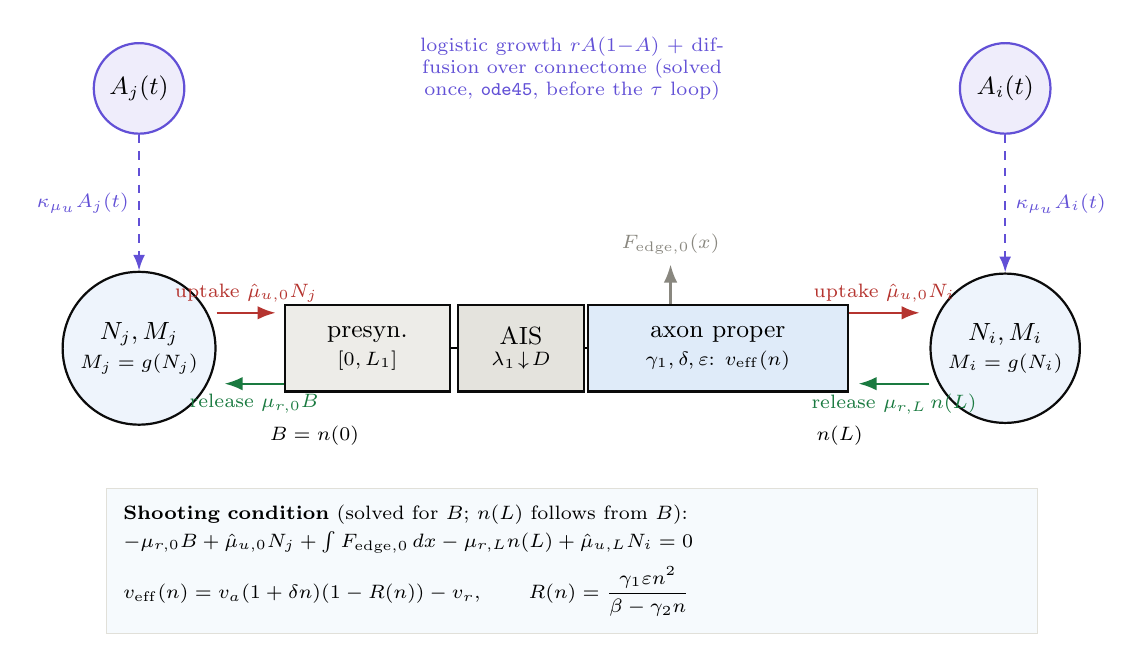
\begin{tikzpicture}[
    >=Latex,
    font=\small,
    node_circ/.style={circle, draw=ntmink, thick, minimum size=1.7cm, fill=ntmblue!8},
    abeta_circ/.style={circle, draw=ntmviolet, thick, minimum size=1.15cm, fill=ntmviolet!10},
    compartment/.style={draw=ntmink, thick, minimum height=1.1cm},
    flux/.style={-{Latex[length=2.3mm]}, thick},
    release/.style={flux, ntmgreen},
    uptake/.style={flux, ntmred},
    couple/.style={-{Latex[length=2mm]}, ntmviolet, dashed, thick},
  ]

  % --- Abeta nodes (top) ---
  \node[abeta_circ] (Aj) at (0,3.3) {$A_j(t)$};
  \node[abeta_circ] (Ai) at (11,3.3) {$A_i(t)$};
  \node[font=\scriptsize, text width=5.4cm, align=center, ntmviolet] at (5.5,3.55)
    {logistic growth $r A(1{-}A)$ + diffusion over connectome (solved once, \texttt{ode45}, before the $\tau$ loop)};

  % --- Main nodes ---
  \node[node_circ] (Nj) at (0,0) {\shortstack{$N_j, M_j$ \\ \scriptsize$M_j=g(N_j)$}};
  \node[node_circ] (Ni) at (11,0) {\shortstack{$N_i, M_i$ \\ \scriptsize$M_i=g(N_i)$}};

  \draw[couple] (Aj) -- (Nj) node[midway, left, font=\scriptsize] {$\kappa_{\muu} A_j(t)$};
  \draw[couple] (Ai) -- (Ni) node[midway, right, font=\scriptsize] {$\kappa_{\muu} A_i(t)$};

  % --- Axon compartments ---
  \node[compartment, minimum width=2.1cm, fill=ntmhair!60] (presyn) at (2.9,0) {\shortstack{presyn. \\ \scriptsize$[0,L_1]$}};
  \node[compartment, minimum width=1.6cm, fill=ntmhair!90] (ais) at (4.85,0) {\shortstack{AIS \\ \scriptsize$\lambda_1\!\downarrow\! D$}};
  \node[compartment, minimum width=3.3cm, fill=ntmblue!15] (axon) at (7.35,0) {\shortstack{axon proper \\ \scriptsize$\gamma_1,\delta,\varepsilon$: $v_{\mathrm{eff}}(n)$}};

  \draw[thick] (presyn) -- (ais);
  \draw[thick] (ais) -- (axon);

  % --- Boundary flux arrows ---
  \draw[uptake] (Nj.east) ++(0,0.45) -- ++(0.75,0) node[midway, above, font=\scriptsize, ntmred] {uptake $\hat\mu_{u,0} N_j$};
  \draw[release] (presyn.west) ++(0,-0.45) -- ++(-0.75,0) node[midway, below, font=\scriptsize, ntmgreen] {release $\mu_{r,0} B$};

  \draw[uptake] (axon.east) ++(0,0.45) -- ++(0.9,0) node[midway, above, font=\scriptsize, ntmred] {uptake $\hat\mu_{u,0} N_i$};
  \draw[release] (Ni.west) ++(0,-0.45) -- ++(-0.9,0) node[midway, below, font=\scriptsize, ntmgreen] {release $\mu_{r,L}\, n(L)$};

  % --- B / n(L) labels ---
  \node[font=\scriptsize, below=0.3cm of presyn.south west, anchor=north west, xshift=-0.3cm] {$B=n(0)$};
  \node[font=\scriptsize, below=0.3cm of axon.south east, anchor=north east, xshift=0.3cm] {$n(L)$};

  % --- distributed source ---
  \draw[->, ntmmuted, thick] (axon.north) ++(-0.6,0) -- ++(0,0.5) node[above, font=\scriptsize, ntmmuted] {$F_{\mathrm{edge},0}(x)$};

  % --- equation panel ---
  \node[draw=ntmhair, fill=ntmblue!4, align=left, font=\scriptsize, text width=11.4cm, inner sep=6pt]
    (eqpanel) at (5.5,-2.7)
    {\textbf{Shooting condition} (solved for $B$; $n(L)$ follows from $B$):\\[2pt]
     $-\mu_{r,0} B + \hat\mu_{u,0} N_j + \int F_{\mathrm{edge},0}\,dx - \mu_{r,L} n(L) + \hat\mu_{u,L} N_i = 0$\\[4pt]
     $v_{\mathrm{eff}}(n) = v_a(1+\delta n)(1-R(n)) - v_r, \qquad R(n)=\dfrac{\gamma_1\varepsilon n^2}{\beta-\gamma_2 n}$};

\end{tikzpicture}
\caption{One edge $j\to i$: three axon compartments, the shooting parameter
$B$ determined by the far-end mass balance, release (green, axon$\to$node)
and uptake (red, node$\to$axon) fluxes, and the A$\beta$ coupling (violet,
dashed) currently active on $\muu$ only. Fluxes on every incident edge sum
into each node's ODE (Section~\ref{sec:node}).}
\label{fig:mechanism}
\end{figure}

Figure~\ref{fig:architecture} shows how the two timescales fit together
across one full run: the A$\beta$ field is solved once, up front, and then
simply read off (never re-solved) at every outer time step, while the
per-edge shooting solve is re-run on \emph{every} edge, at every outer time
step (and twice, at predictor and corrector states, for the first 50 steps).

\begin{figure}[htbp]
\centering
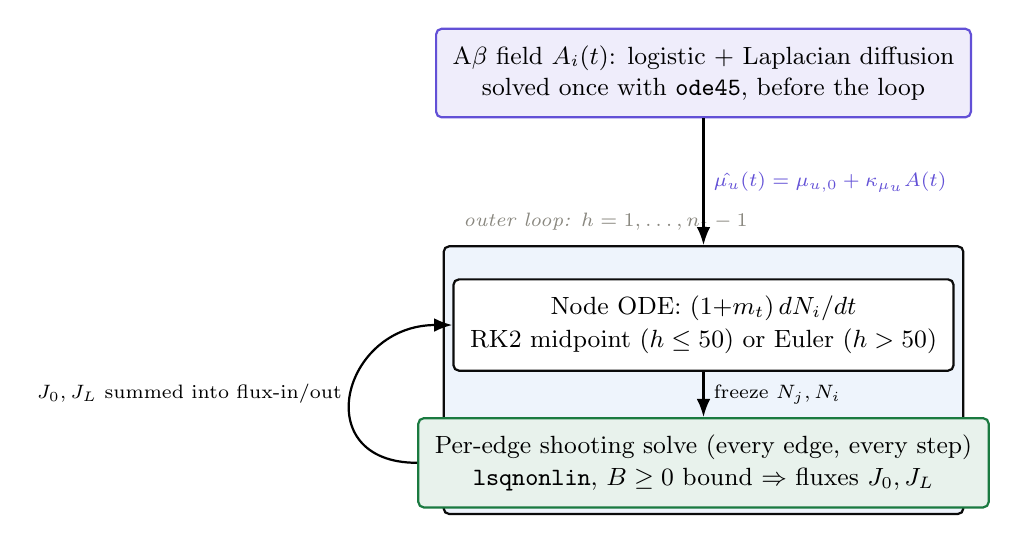
\begin{tikzpicture}[
    >=Latex,
    font=\small,
    box/.style={draw=ntmink, thick, rounded corners=2pt, align=center, minimum height=0.95cm, inner sep=6pt},
    once/.style={box, fill=ntmviolet!10, draw=ntmviolet},
    loopbox/.style={box, fill=ntmblue!8},
    innerbox/.style={box, fill=ntmgreen!10, draw=ntmgreen, minimum width=6.6cm},
    arr/.style={-{Latex[length=2.3mm]}, thick},
  ]

  \node[once, minimum width=6.6cm] (abeta) at (0,5.2) {\shortstack{A$\beta$ field $A_i(t)$: logistic + Laplacian diffusion \\ solved once with \texttt{ode45}, before the loop}};

  \node[loopbox, minimum width=6.6cm, minimum height=3.4cm] (loop) at (0,1.3) {};
  \node[font=\scriptsize\itshape, ntmmuted, anchor=south west] at (loop.north west) [xshift=4pt, yshift=2pt] {outer loop: $h=1,\dots,n_t-1$};

  \node[box, minimum width=5.6cm, fill=white] (nodeode) at (0,2.0) {\shortstack{Node ODE: $(1{+}m_t)\,dN_i/dt$ \\ RK2 midpoint ($h\le 50$) or Euler ($h>50$)}};

  \node[innerbox] (shoot) at (0,0.25) {\shortstack{Per-edge shooting solve (every edge, every step) \\ \texttt{lsqnonlin}, $B\ge 0$ bound $\Rightarrow$ fluxes $J_0, J_L$}};

  \draw[arr] (abeta) -- (loop.north -| abeta) node[midway, right, font=\scriptsize, ntmviolet] {$\hat\muu(t)=\mu_{u,0}+\kappa_{\muu}A(t)$};
  \draw[arr] (nodeode) -- (shoot) node[midway, right, font=\scriptsize] {freeze $N_j,N_i$};
  \draw[arr] (shoot.west) .. controls +(-1.4,0) and +(-1.4,0) .. (nodeode.west)
      node[midway, left, font=\scriptsize] {$J_0,J_L$ summed into flux-in/out};

\end{tikzpicture}
\caption{Two-timescale solve architecture. A$\beta$ is solved exactly once
and only read thereafter (one-way coupling); the per-edge shooting solve is
the inner loop re-run at every outer node-level time step.}
\label{fig:architecture}
\end{figure}

% =========================================================================
\section{Parameter summary}
% =========================================================================

\begin{table}[h]
\centering
\caption{Parameters as named in \texttt{call\_NTM\_brandontest.m} / \texttt{NetworkFluxCalculator\_Neu.m}.}
\begin{tabularx}{\textwidth}{@{} p{3.6cm} c X @{}}
\toprule
Code name & Symbol & Role \\
\midrule
\texttt{beta} & $\beta$ & Fragmentation ($M\to N$); also sets $n^\star=\sqrt{\beta/(\gamma_1\varepsilon)}$ \\
\texttt{gamma1} & $\gamma_1$ & Soluble--soluble aggregation \\
\texttt{gamma2} & $\gamma_2$ & Soluble--insoluble aggregation (default $0$) \\
\texttt{delta} & $\delta$ & Motor-crowding velocity boost \\
\texttt{epsilon} & $\varepsilon$ & Aggregation$\to$velocity coupling \\
\texttt{mu\_r\_0}, \texttt{mu\_r\_L} & $\mu_{r,0},\mu_{r,L}$ & Release rate, source/target end \\
\texttt{mu\_u\_0}, \texttt{mu\_u\_L} & $\mu_{u,0},\mu_{u,L}$ & Uptake rate, source/target end \\
\texttt{F\_edge\_0} & $F_{\mathrm{edge},0}$ & Distributed-source strength \\
\texttt{frac} & $\phi$ & Advective/diffusive split in the axon ODE \\
\texttt{alpha} & $\alpha$ & Linear tau growth at nodes \\
\texttt{r} & $r$ & A$\beta$ logistic growth rate \\
\texttt{Dif} & $D$ & A$\beta$ diffusion coefficient over the connectome \\
\texttt{coupling\_term} & --- & Which of $\{\mu_u,\mu_r,\delta,\varepsilon\}$ read A$\beta$ \\
\texttt{kappa\_mu\_u}, \texttt{kappa\_mu\_r},\newline\texttt{kappa\_delta}, \texttt{kappa\_epsilon} & $\kappa_{(\cdot)}$ & A$\beta$ coupling strengths \\
\bottomrule
\end{tabularx}
\end{table}

\vspace{1em}
{\footnotesize Release/uptake mechanics per Barron et al.\ 2026 (bioRxiv), Fig.~1 and eqs.~1--5,
mapped to this repository's variable names. The A$\beta$ sub-model and its
coupling into tau kinetic parameters are this repository's own extension and
are not part of that source.}

\end{document}
